\documentclass{standalone}
\usepackage{tikz}

\begin{document}
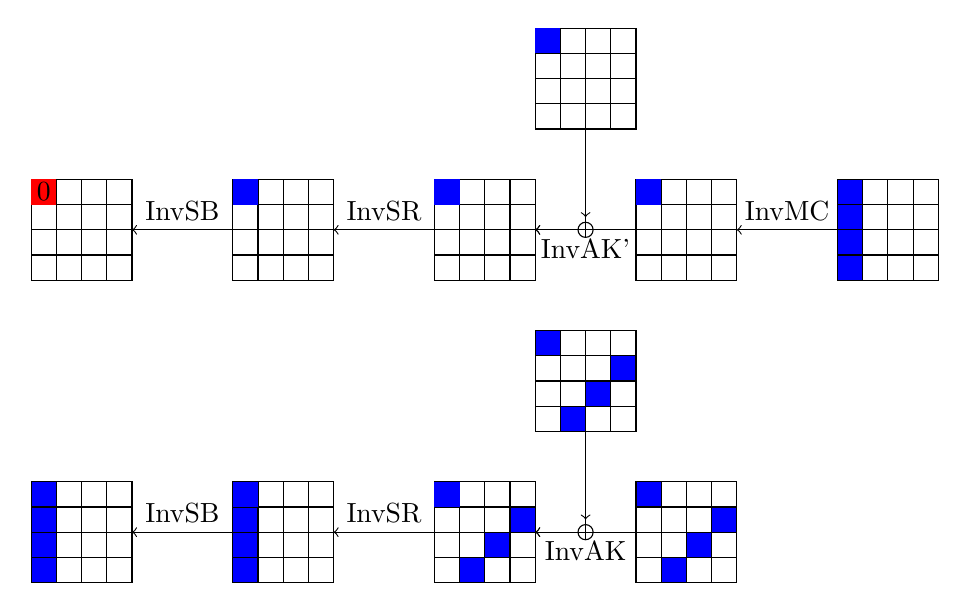
\begin{tikzpicture}[scale=0.32]
  \begin{scope}[yshift=6cm,xshift=-8cm]
  
    \draw (0,0) rectangle (4,4);
    \draw (0,1) -- +(4,0);
    \draw (0,2) -- +(4,0);
    \draw (0,3) -- +(4,0);
    \draw (1,0) -- +(0,4);
    \draw (2,0) -- +(0,4);
    \draw (3,0) -- +(0,4);
    % \path (6,2) node {$\delta$-set};
    \draw[<-] (4,2) -- node[above]{InvSB} ++(4,0);
      \fill[red] (0, 3) rectangle ++(1,1);
     \path[shift={(0.5,0.5)}] (0,3) node {$0$};
  \end{scope}

    \begin{scope}[yshift=6cm,xshift=0cm]
    % \path[shift={(0.5,0.5)}] (0,3) node {$\star$};
    \draw (0,0) rectangle (4,4);
    \draw (0,1) -- +(4,0);
    \draw (0,2) -- +(4,0);
    \draw (0,3) -- +(4,0);
    \draw (1,0) -- +(0,4);
    \draw (2,0) -- +(0,4);
    \draw (3,0) -- +(0,4);
    % \path (6,2) node {$\delta$-set};
          \draw[<-] (4,2) -- node[above]{InvSR} ++(4,0);
    % \draw (0,2) -- ++(-1.5,0) -- +(0,-6.4);
      \fill[blue] (0, 3) rectangle ++(1,1);
  \end{scope}

      \begin{scope}[yshift=6cm,xshift=8cm]
    % \path[shift={(0.5,0.5)}] (0,3) node {$\star$};
    \draw (0,0) rectangle (4,4);
    \draw (0,1) -- +(4,0);
    \draw (0,2) -- +(4,0);
    \draw (0,3) -- +(4,0);
    \draw (1,0) -- +(0,4);
    \draw (2,0) -- +(0,4);
    \draw (3,0) -- +(0,4);
        \draw[<-] (4,2) -- ++(4,0);
          \draw[<-] (4,2) -- node[below]{InvAK'} ++(4,0);
            \draw (6,2) circle (0.3);
    % \path (6,2) node {$\delta$-set};
    % \draw (0,2) -- ++(-1.5,0) -- +(0,-6.4);
      \fill[blue] (0, 3) rectangle ++(1,1);
  \end{scope}

        \begin{scope}[yshift=6cm,xshift=16cm]
    % \path[shift={(0.5,0.5)}] (0,3) node {$0$};
    \draw (0,0) rectangle (4,4);
    \draw (0,1) -- +(4,0);
    \draw (0,2) -- +(4,0);
    \draw (0,3) -- +(4,0);
    \draw (1,0) -- +(0,4);
    \draw (2,0) -- +(0,4);
    \draw (3,0) -- +(0,4);
    % \path (6,2) node {$\delta$-set};
    % \draw (0,2) -- ++(-1.5,0) -- +(0,-6.4);
    \fill[blue] (0, 3) rectangle ++(1,1);
 \draw[<-] (4,2) -- node[above]{InvMC} ++(4,0);
  \end{scope}

    \begin{scope}[yshift=12cm,xshift=12cm]
    % \path[shift={(0.5,0.5)}] (0,3) node {$\star$};
    \draw (0,0) rectangle (4,4);
    \draw (0,1) -- +(4,0);
    \draw (0,2) -- +(4,0);
    \draw (0,3) -- +(4,0);
    \draw (1,0) -- +(0,4);
    \draw (2,0) -- +(0,4);
    \draw (3,0) -- +(0,4);
    % \path (6,2) node {$\delta$-set};
    % \draw (0,2) -- ++(-1.5,0) -- +(0,-6.4);

    \draw (2,0) -- ++(0, -4.3);
        \draw[->] (2,0) -- ++(0, -3.5);

    \fill[blue] (0, 3) rectangle ++(1,1);

  \end{scope}


      \begin{scope}[yshift=6cm,xshift=24cm]
        \fill[blue] (0, 0) rectangle ++(1,4);
    % \path[shift={(0.5,0.5)}] (0,3) node {$\star$};
    \draw (0,0) rectangle (4,4);
    \draw (0,1) -- +(4,0);
    \draw (0,2) -- +(4,0);
    \draw (0,3) -- +(4,0);
    \draw (1,0) -- +(0,4);
    \draw (2,0) -- +(0,4);
    \draw (3,0) -- +(0,4);
    % \path (6,2) node {$\delta$-set};
    % \draw (0,2) -- ++(-1.5,0) -- +(0,-6.4);

    % \draw (2,0) -- ++(0, -4.3);
    %     \draw[->] (2,0) -- ++(0, -3.5);



  \end{scope}










\begin{scope}[yshift=-12cm]
 \begin{scope}[yshift=6cm,xshift=-8cm]
    \fill[blue] (0, 3) rectangle ++(1,1);
    \fill[blue] (0, 2) rectangle ++(1,1);
    \fill[blue] (0, 1) rectangle ++(1,1);
    \fill[blue] (0, 0) rectangle ++(1,1);
  
    \draw (0,0) rectangle (4,4);
    \draw (0,1) -- +(4,0);
    \draw (0,2) -- +(4,0);
    \draw (0,3) -- +(4,0);
    \draw (1,0) -- +(0,4);
    \draw (2,0) -- +(0,4);
    \draw (3,0) -- +(0,4);
    % \path (6,2) node {$\delta$-set};
    \draw[<-] (4,2) -- node[above]{InvSB} ++(4,0);
      % \fill[red] (0, 3) rectangle ++(1,1);
     % \path[shift={(0.5,0.5)}] (0,3) node {$0$};
  \end{scope}

    \begin{scope}[yshift=6cm,xshift=0cm]
    % \path[shift={(0.5,0.5)}] (0,3) node {$\star$};
    \fill[blue] (0, 3) rectangle ++(1,1);
    \fill[blue] (0, 2) rectangle ++(1,1);
    \fill[blue] (0, 1) rectangle ++(1,1);
    \fill[blue] (0, 0) rectangle ++(1,1);

    \draw (0,0) rectangle (4,4);
    \draw (0,1) -- +(4,0);
    \draw (0,2) -- +(4,0);
    \draw (0,3) -- +(4,0);
    \draw (1,0) -- +(0,4);
    \draw (2,0) -- +(0,4);
    \draw (3,0) -- +(0,4);
    % \path (6,2) node {$\delta$-set};
          \draw[<-] (4,2) -- node[above]{InvSR} ++(4,0);
    % \draw (0,2) -- ++(-1.5,0) -- +(0,-6.4);
      \fill[blue] (0, 3) rectangle ++(1,1);
  \end{scope}

      \begin{scope}[yshift=6cm,xshift=8cm]
        \fill[blue] (0, 3) rectangle ++(1,1);
    \fill[blue] (3, 2) rectangle ++(1,1);
    \fill[blue] (2, 1) rectangle ++(1,1);
    \fill[blue] (1, 0) rectangle ++(1,1);
    % \path[shift={(0.5,0.5)}] (0,3) node {$\star$};
    \draw (0,0) rectangle (4,4);
    \draw (0,1) -- +(4,0);
    \draw (0,2) -- +(4,0);
    \draw (0,3) -- +(4,0);
    \draw (1,0) -- +(0,4);
    \draw (2,0) -- +(0,4);
    \draw (3,0) -- +(0,4);
        \draw[<-] (4,2) -- ++(4,0);
          \draw[<-] (4,2) -- node[below]{InvAK} ++(4,0);
            \draw (6,2) circle (0.3);
    % \path (6,2) node {$\delta$-set};
    % \draw (0,2) -- ++(-1.5,0) -- +(0,-6.4);
      \fill[blue] (0, 3) rectangle ++(1,1);
  \end{scope}

        \begin{scope}[yshift=6cm,xshift=16cm]
    % \path[shift={(0.5,0.5)}] (0,3) node {$0$};
        \fill[blue] (0, 3) rectangle ++(1,1);
    \fill[blue] (3, 2) rectangle ++(1,1);
    \fill[blue] (2, 1) rectangle ++(1,1);
    \fill[blue] (1, 0) rectangle ++(1,1);
    \draw (0,0) rectangle (4,4);
    \draw (0,1) -- +(4,0);
    \draw (0,2) -- +(4,0);
    \draw (0,3) -- +(4,0);
    \draw (1,0) -- +(0,4);
    \draw (2,0) -- +(0,4);
    \draw (3,0) -- +(0,4);
    % \path (6,2) node {$\delta$-set};
    % \draw (0,2) -- ++(-1.5,0) -- +(0,-6.4);
    % \fill[blue] (0, 3) rectangle ++(1,1);
 % \draw[<-] (4,2) -- node[above]{InvMC} ++(4,0);
  \end{scope}

    \begin{scope}[yshift=12cm,xshift=12cm]
    % \path[shift={(0.5,0.5)}] (0,3) node {$\star$};
    \fill[blue] (0, 3) rectangle ++(1,1);
    \fill[blue] (3, 2) rectangle ++(1,1);
    \fill[blue] (2, 1) rectangle ++(1,1);
    \fill[blue] (1, 0) rectangle ++(1,1);

    \draw (0,0) rectangle (4,4);
    \draw (0,1) -- +(4,0);
    \draw (0,2) -- +(4,0);
    \draw (0,3) -- +(4,0);
    \draw (1,0) -- +(0,4);
    \draw (2,0) -- +(0,4);
    \draw (3,0) -- +(0,4);
    % \path (6,2) node {$\delta$-set};
    % \draw (0,2) -- ++(-1.5,0) -- +(0,-6.4);

    \draw (2,0) -- ++(0, -4.3);
        \draw[->] (2,0) -- ++(0, -3.5);



  \end{scope}


  %     \begin{scope}[yshift=6cm,xshift=24cm]
  %       \fill[blue] (0, 0) rectangle ++(1,4);
  %   % \path[shift={(0.5,0.5)}] (0,3) node {$\star$};
  %   \draw (0,0) rectangle (4,4);
  %   \draw (0,1) -- +(4,0);
  %   \draw (0,2) -- +(4,0);
  %   \draw (0,3) -- +(4,0);
  %   \draw (1,0) -- +(0,4);
  %   \draw (2,0) -- +(0,4);
  %   \draw (3,0) -- +(0,4);
  %   % \path (6,2) node {$\delta$-set};
  %   % \draw (0,2) -- ++(-1.5,0) -- +(0,-6.4);

  %   % \draw (2,0) -- ++(0, -4.3);
  %   %     \draw[->] (2,0) -- ++(0, -3.5);



  % \end{scope}
  \end{scope}
  
\end{tikzpicture}
\end{document}
